\chapter{Electromagnetism}
\label{p:em:em11}

\section{Introduction}

Electromagnetism describes the interaction between charges, currents and the electric and magnetic fields which they give rise to. An electric current creates a magnetic field and a changing magnetic field will create a flow of charge. This relationship between electricity and magnetism has resulted in the invention of many devices which are useful to humans.\\
\chapterstartvid{VPlwi}
\section{Magnetic field associated with a current}
%\begin{syllabus}
%\item Provide evidence for the existence of a magnetic field near a current carrying wire.
%\item Use the Right Hand Rule to determine the magnetic field associated with: (a) a straight current carrying wire, (b) a current carrying loop of wire and (c) a solenoid.
%\item Note: A simple form of evidence for the existence of a magnetic field near a current carrying wire is that a compass needle placed near the wire will deflect (link to Grade 10).
%\item Note: In all situations involving magnetic fields and moving charges, only the Right hand Rule is used to find directions.  This is done to reduce confusion amongst learners who may struggle trying to remember which hand and which fingers to use if there is more than one rule.
%\item Suggestions: Explain the right hand rule only!
%\item Suggestions: show notation and field directions then have a suggestion/exercise that they try to figure out a rule (hint - use hands and fingers) to determine which way the field goes
%\item Suggestions: Try to include possible questions that help test the above content
%\end{syllabus}
If you hold a compass near a wire through which current is
flowing, the needle on the compass will be deflected.
%\begin{center}
%\begin{pspicture}(-0.8,-2)(10,3.4)
%\psgrid[gridcolor=gray]
%\def\comp{\pscircle(0,0){0.5}\uput{0.3cm}[u](0,0.25){N}\uput{0.3cm}[d](0,-0.25){compass}}
%\uput[u](2.5,3){conductor} \psline[linewidth=2pt](1,3)(4,3)
%\psline(4,3)(4,0) \battery(1,0)(4,0){} \psline(1,0)(1,0.6)
%\psline(1,1.4)(1,3)
%\rput(2.5,2){\psset{unit=0.8}\comp\rput(0,0){\psline{->}(0,-0.25)(0,0.25)}}
%\uput[l](1,1){\parbox{1.5cm}{no current is flowing}}
%\uput[d](2.5,-0.4){\parbox[l]{4cm}{There is no deflection on the
%compass when there is no current flowing in the conductor.}}

%\rput(6,0){\uput[u](2.5,3){conductor}
%\psline[linewidth=2pt](1,3)(4,3) \psline(4,3)(4,0)
%\battery(1,0)(4,0){} \psline(1,0)(1,3)
%\rput(2.5,2){\psset{unit=0.8}\comp\rput{45}(0,0){\psline{->}(0,-0.25)(0,0.25)}}
%\uput[l](1,1){\parbox{1.5cm}{current is flowing}}
%\psline{->}(1.2,0.6)(1.2,1.4) \uput[d](2,-0.4){\parbox[l]{4cm}{The
%compass needle deflects when there \textit{is} current flowing in
%the conductor.}} }
%\end{pspicture}
%\end{center}

Since compasses work by pointing along magnetic field lines, this means that there must be a magnetic field near the wire through which the current is flowing.

%\Activity{Case Study}{Magnetic field near a current carrying conductor}{

%\begin{center}
%\begin{pspicture}(-1.8,-2)(11,3.4)
%\psgrid[gridcolor=gray]
%\def\comp{\pscircle(0,0){0.5}\uput{0.3cm}[u](0,0.25){N}\uput{0.3cm}[d](0,-0.25){compass}}
%\rput(-1,0){ \uput[u](2.5,3){conductor}
%\psline[linewidth=2pt](1,3)(4,3) \psline(4,3)(4,0)
%\battery(1,0)(4,0){} \psline(1,0)(1,3)
%\rput(2.5,2){\psset{unit=0.8}\comp\rput{45}(0,0){\psline{->}(0,-0.25)(0,0.25)}}
%\uput[l](1,1){\parbox{1.5cm}{direction of current}}
%\psline{->}(1.2,0.6)(1.2,1.4)
%\uput[d](2,-0.4){\parbox[l]{5.5cm}{When the battery is connected
%as shown, the compass needle is deflected to the left.}} }

%\rput(6,0){\uput[u](2.5,3){conductor}
%\psline[linewidth=2pt](1,3)(4,3) \psline(4,3)(4,0)
%\rput{180}(5,0){\battery(1,0)(4,0){}} \psline(1,0)(1,3)
%\rput(2.5,2){\psset{unit=0.8}\comp}
%\uput[l](1,1){\parbox{1.5cm}{direction of current}}
%\psline{<-}(1.2,0.6)(1.2,1.4)
%\uput[d](2,-0.4){\parbox[l]{5.5cm}{What do you think will happen
%if the direction of the current is reversed as shown?}} }
%\end{pspicture}
%\end{center}
%}

The magnetic field produced by an electric current is always
oriented perpendicular to the direction of the current flow. When
we are drawing directions of magnetic fields and currents, we use
the symbols $\odot$ and $\otimes$.
The symbol \nequ{\odot} represents an
arrow that is coming out of the page and the symbol \nequ{\otimes}
represents an arrow that is going into the page.
\begin{IFact}{The Danish physicist Hans Christian Oersted was lecturing one day in 1820 on the possibility of electricity and magnetism being related to one another, and in the process demonstrated it conclusively by experiment in front of his whole class. By passing an electric current through a metal wire suspended above a magnetic compass, Oersted was able to produce a definite motion of the compass needle in response to the current. What began as a guess at the start of the class session was confirmed as fact at the end. Needless to say, Oersted had to revise his lecture notes for future classes. His discovery paved the way for a whole new branch of science - electromagnetism.}
\end{IFact}
It is easy to remember the meanings of the symbols if you think of
an arrow with a head and a tail.

\begin{center}
\begin{pspicture}(0,-0.4)(3,0.4)
%\psgrid[gridcolor=gray]
\psline[arrows=<-<<,arrowsize=0.2cm](0,0)(3,0)
\end{pspicture}
\end{center}

When the arrow is coming out of the page, you see the point of the
arrow ($\odot$). When the arrow is going into the page, you see
the tail of the arrow ($\otimes$).

The direction of the magnetic field around the current carrying
conductor is shown in Figure~\ref{p:em:em11:mfccc}.

\begin{figure}[htbp]
\begin{center}
\begin{pspicture}(0,-0.6)(10,4.2)
%\psgrid[gridcolor=gray]
\psarc[arrowsize=6pt]{->}(2,2){2}{90}{90}
\psarc[arrowsize=6pt]{->}(2,2){1.5}{90}{90}
\psarc[arrowsize=6pt]{->}(2,2){1}{90}{90}
\psarc[arrowsize=6pt]{->}(2,2){0.5}{90}{90} \rput(2,2){\Large
$\odot$} \psarc[arrowsize=6pt]{<-}(8,2){2}{90}{90}
\psarc[arrowsize=6pt]{<-}(8,2){1.5}{90}{90}
\psarc[arrowsize=6pt]{<-}(8,2){1}{90}{90}
\psarc[arrowsize=6pt]{<-}(8,2){0.5}{90}{90} \rput(8,2){\Large
$\otimes$} \uput[d](2,0){(a)} \uput[d](8,0){(b)}
\end{pspicture}
\caption{Magnetic field around a conductor when you look at the
conductor from one end. (a) Current flows out of the page and the
magnetic field is counter clockwise. (b) Current flows into the
page and the magnetic field is clockwise.} \label{p:em:em11:mfccc}
\end{center}
\end{figure}

\begin{figure}[htbp]
\begin{center}
\begin{pspicture}(0,0)(10,3)
%\psgrid[gridcolor=gray]
\psline[linewidth=2pt](1,2)(4,2)
\arrowLine[arrowsize=6pt,linewidth=2pt](1,2)(4,2){1}
\multirput(1.5,1.4)(1,0){3}{\Large $\otimes$}
\multirput(1.5,2.6)(1,0){3}{\Large $\odot$}
\pcline[offset=0.2cm]{->}(1,0.5)(1,1.5) \aput{:U}{current flow}
\psline(1,2)(1,0) \battery(1,0)(4,0){} \psline(4,0)(4,2)
\rput(5,0){ \arrowLine[arrowsize=6pt,linewidth=2pt](4,2)(1,2){1}
\psline[linewidth=2pt](1,2)(4,2)
\multirput(1.5,2.6)(1,0){3}{\Large $\otimes$}
\multirput(1.5,1.4)(1,0){3}{\Large $\odot$}
\pcline[offset=0.2cm]{<-}(1,0.5)(1,1.5) \aput{:U}{current flow}
\psline(1,2)(1,0) \rput{180}(5,0){\battery(1,0)(4,0){}}
\psline(4,0)(4,2) }
\end{pspicture}
\caption{Magnetic fields around a conductor looking down on the
conductor. (a) Current flows clockwise. (b) current flows counter clockwise.} \label{p:em:em11:mfccc2}
\end{center}
\end{figure}

\pagebreak
\Activity{Case Study}{Direction of a magnetic field}{Using the directions given
in Figure~\ref{p:em:em11:mfccc} and Figure~\ref{p:em:em11:mfccc2} try to find a rule that easily tells you the direction of the
magnetic field.

Hint: Use your fingers. Hold the wire in your hands and try to
find a link between the direction of your thumb and the direction
in which your fingers curl.}

\begin{center}
\begin{pspicture}(0,0)(5,4.5)
%\psgrid[gridcolor=gray]
\psline[linewidth=6pt]{->}(2.5,0)(2.5,4.5)
\def\field{\psellipse[linecolor=gray](2.5,0.5)(1,0.20)
\psline[linecolor=gray,arrowsize=5pt]{->}(2.49,0.3)(2.51,0.3)
\psline[linewidth=6pt](2.5,0.6)(2.5,0.8)}
\multirput(0,0.25)(0,0.5){7}{\field}
\uput[r](4,3){\parbox[l]{4cm}{The magnetic field around a current
carrying conductor.}}
\end{pspicture}
\end{center}

There is a simple method of finding the relationship between the
direction of the current flowing in a conductor and the direction
of the magnetic field around the same conductor. The method is
called the \textit {Right Hand Rule}. Simply stated, the right
hand rule says that the magnetic field lines produced by a
current-carrying wire will be oriented in the same direction as the
curled fingers of a person's right hand (in the "hitchhiking"
position), with the thumb pointing in the direction of the current
flow.

\begin{figure}[htbp]
\begin{center}
\begin{pspicture}(-4,-2)(1.8,2.4)
%\psgrid
\rput(0,0){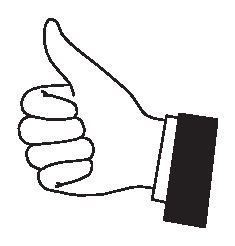
\includegraphics{../right-hand-rule.eps}}
\pcline{->}(0,1)(0,2) \bput{:U}{\parbox{1.5cm}{direction of
current}}
\multirput(0,0)(0,0.5){4}{\psarc{->}(-1.8,0){1}{180}{270}}
\pcline[linestyle=none](-3,-1)(-3,1) \aput{:U}{direction of
magnetic field}
\end{pspicture}
\caption{The Right Hand Rule.}
\end{center}
\end{figure}

\Activity{Case Study}{The Right Hand Rule}{Use the Right Hand Rule to draw in
the directions of the magnetic fields for the following conductors
with the currents flowing in the directions shown by the arrows.
The first problem has been completed for you.

\begin{center}
\begin{tabular}{lclclclc}%lclc}%lclclclclclcl}
1. &
\begin{pspicture}(-1,-1)(1,1)
%\psgrid
\psline{<-}(-1,0)(1,0) \multirput(-0.5,0.4)(0.5,0){3}{$\otimes$}
\multirput(-0.5,-0.4)(0.5,0){3}{$\odot$}
\end{pspicture} &
2. &
\begin{pspicture}(-1,-1)(1,1)
%\psgrid
\rput{30}{\psline{<-}(-1,0)(1,0)}
\end{pspicture} &
3. &
\begin{pspicture}(-1,-1)(1,1)
%\psgrid
\rput{60}{\psline{<-}(-1,0)(1,0)}
\end{pspicture}&
4. &
\begin{pspicture}(-1,-1)(1,1)
%\psgrid
\rput{90}{\psline{<-}(-1,0)(1,0)}
\end{pspicture}
\\
5. &
\begin{pspicture}(-1,-1)(1,1)
%\psgrid
\rput{120}{\psline{<-}(-1,0)(1,0)}
\end{pspicture} &
6. &
\begin{pspicture}(-1,-1)(1,1)
%\psgrid
\rput{150}{\psline{<-}(-1,0)(1,0)}
\end{pspicture} &
7. &
\begin{pspicture}(-1,-1)(1,1)
%\psgrid
\rput{180}{\psline{<-}(-1,0)(1,0)}
\end{pspicture} &
8. &
\begin{pspicture}(-1,-1)(1,1)
%\psgrid
\rput{210}{\psline{<-}(-1,0)(1,0)}
\end{pspicture} \\
9. &
\begin{pspicture}(-1,-1)(1,1)
%\psgrid
\rput{240}{\psline{<-}(-1,0)(1,0)}
\end{pspicture} &
10. &
\begin{pspicture}(-1,-1)(1,1)
%\psgrid
\rput{270}{\psline{<-}(-1,0)(1,0)}
\end{pspicture} &
11. &
\begin{pspicture}(-1,-1)(1,1)
%\psgrid
\rput{300}{\psline{<-}(-1,0)(1,0)}
\end{pspicture} &
12. &
\begin{pspicture}(-1,-1)(1,1)
%\psgrid
\rput{330}{\psline{<-}(-1,0)(1,0)}
\end{pspicture}
\end{tabular}
\end{center}
}

\begin{g_experiment}{Magnetic field around a current carrying conductor}{
\textbf{Apparatus: } 
\begin{enumerate}
\item one 9V battery with holder
\item two hookup wires with alligator clips
\item compass
\item stop watch
\end{enumerate}
\textbf{Method: }
\begin{enumerate}
\item Connect your wires to the battery leaving one end of each wire unconnected so that the circuit is not closed.
\item One student should be in charge of limiting the current flow to 10 seconds. This is to preserve battery life as well as to prevent overheating of the wires and battery contacts.
\item Place the compass close to the wire.
\item Close the circuit and observe what happens to the compass.
\item Reverse the polarity of the battery and close the circuit. Observe what happens to the compass.
\end{enumerate}
\textbf{Conclusions: }\\
Use your observations to answer the following questions:
\begin{enumerate}
\item Does a current flowing in a wire generate a magnetic field?
\item Is the magnetic field present when the current is not flowing?
\item Does the direction of the magnetic field produced by a current in a wire depend on the direction of the current flow?
\item How does the direction of the current affect the magnetic field?
\end{enumerate}
}
\end{g_experiment}
\Activity{Case Study}{Magnetic field around a loop of conductor}{Consider two
loops made from a conducting material, which carry currents (in opposite directions) and are placed in the plane
of the page. By using the Right Hand Rule, draw what you think the magnetic field would look
like at different points around each of the two
loops. Loop 1 has the current flowing in a counter-clockwise
direction, while loop 2 has the current flowing in a clockwise
direction.

\begin{center}
\begin{pspicture}(-2,-1.4)(6,1.8)
%\psgrid
\psset{unit=1.5} \psellipse(0,0)(1,0.5)
\psline{<-}(-0.2,0.6)(0.2,0.6) \psline{<-}(-1.2,-0.2)(-1.2,0.2)
\psline{->}(-0.2,-0.6)(0.2,-0.6) \psline{->}(1.2,-0.2)(1.2,0.2)
\uput[u](0,0.6){direction of current} \uput[d](0,-0.6){direction
of current} \rput(0,0){loop 1}

\rput(3,0){\psellipse(0,0)(1,0.5) \psline{->}(-0.2,0.6)(0.2,0.6)
\psline{->}(-1.2,-0.2)(-1.2,0.2) \psline{<-}(-0.2,-0.6)(0.2,-0.6)
\psline{<-}(1.2,-0.2)(1.2,0.2) \uput[u](0,0.6){direction of
current} \uput[d](0,-0.6){direction of current} \rput(0,0){loop 2}
}
\end{pspicture}

\end{center}

}

If you make a loop of current carrying conductor, then the
direction of the magnetic field is obtained by applying the Right
Hand Rule to different points in the loop.

\begin{center}
\begin{pspicture}(-2,-2)(2,2)
%\psgrid
\psarc{->}(0,0){1.5}{0}{179} \psarc{->}(0,0){1.5}{180}{359}
\degrees[1.1] \multido{\n=0.0+.1}{11} { \rput(1.3;\n){$\odot$}
\rput(1.7;\n){$\otimes$} } \uput[r](2,0){\parbox[l]{5cm}{The
directions of the magnetic field around a loop of current carrying
conductor with the current flowing in a counter-clockwise
direction is shown.}}
\end{pspicture}
\end{center}

If we now add another loop with the current in the same direction, then the magnetic field around each
loop can be added together to create a stronger magnetic field. A coil of many such loops is called a \textit{solenoid}. The magnetic field pattern around a solenoid is similar to the magnetic field pattern around the bar magnet that you studied in Grade 10, which had a definite north and south pole.

\begin{figure}[htbp]
\begin{center}
\begin{pspicture}(-3,-4.6)(3,2.4)
%\psgrid
\rput(0,0){
\includegraphics[width=6.8cm]{../magnetic-field.eps}}
\rput(0,0){\psCoil[coilwidth=1cm,coilheight=0.5]{-1800}{1800}}
\psline(-1.75,0.5)(-2.5,0.5)(-2.5,-4) \battery(-2.5,-4)(2.5,-4){}
\psline(2.5,-4)(2.5,0.5)(1.75,0.5) \pcline{<-}(-2,-3.8)(-1,-3.8)
\aput{:U}{current flow}
\end{pspicture}
\caption{Magnetic field around a solenoid.}
\end{center}
\end{figure}

\subsection{Real-world applications}
\subsubsection{Electromagnets}
An \textit{electromagnet} is a piece of wire intended to generate
a magnetic field with the passage of electric current through it.
Though all current-carrying conductors produce magnetic fields, an
electromagnet is usually constructed in such a way as to maximise
the strength of the magnetic field it produces for a special
purpose. Electromagnets are commonly used in research,
industry, medical, and consumer products. An example of a commonly used electromagnet is in security doors, e.g.\@{} on shop doors which open automatically.

As an electrically-controllable magnet, electromagnets form part of a wide variety of "electromechanical" devices:
machines that produce a mechanical force or motion through electrical
power. Perhaps the most obvious example of such a machine is the
\textit{electric motor} which will be described in detail in Grade
12. Other examples of the use of electromagnets are electric bells, relays, loudspeakers and scrapyard cranes.

\begin{g_experiment}{Electromagnets}{\textbf{Aim: } A magnetic field is created when an electric current flows through a wire. A single wire does not produce a strong magnetic field, but a wire coiled around an iron core does. We will investigate this behaviour.\\
\textbf{Apparatus: }
\begin{enumerate}
\item a battery and holder
\item a length of wire
\item a compass
\item a few nails
\end{enumerate}
\textbf{Method: }
\begin{enumerate}
\item If you have not done the previous experiment in this chapter do it now.
\item Bend the wire into a series of coils before attaching it to the battery. Observe what happens to the deflection of the needle on the compass. Has the deflection of the compass grown stronger?
\item Repeat the experiment by changing the number and size of the coils in the wire. Observe what happens to the deflection on the compass.
\item Coil the wire around an iron nail and then attach the coil to the battery. Observe what happens to the deflection of the compass needle.
\end{enumerate}
\textbf{Conclusions: }
\begin{enumerate}
\item Does the number of coils affect the strength of the magnetic field?
\item Does the iron nail increase or decrease the strength of the magnetic field?
\end{enumerate}
}
\end{g_experiment}

\Exercise{Magnetic Fields}{
  \begin{enumerate}
  \item Give evidence for the existence of a magnetic field near a current carrying wire.
  \item Describe how you would use your right hand to determine the direction of a magnetic field around a current carrying conductor.
  \item Use the Right Hand Rule to determine the direction of the magnetic field for the following situations:
    \begin{enumerate}
    \item
      \begin{center}
        \scalebox{.8}{
          \begin{pspicture}(-3,-4.6)(3,2.4)
            % \psgrid
            \rput(0,0){
\includegraphics[width=6.8cm]{../magnetic-field.eps}}
            \rput(0,0){\psCoil[coilwidth=1cm,coilheight=0.5]{-1800}{1800}}
            \psline(-1.75,0.5)(-2.5,0.5)(-2.5,-4)
            \rput{180}(0,-8){\battery(-2.5,-4)(2.5,-4){}}
            \psline(2.5,-4)(2.5,0.5)(1.75,0.5) \pcline{->}(-2,-3.8)(-1,-3.8)
            \aput{:U}{current flow}
          \end{pspicture}}
      \end{center}
    \item
      \begin{center}
        \scalebox{.8}{
          \begin{pspicture}(-3,-4.6)(3,2.4)
            % \psgrid
            \rput(0,0){
\includegraphics[width=6.8cm]{../magnetic-field.eps}}
            \rput(0,0){\psCoil[coilwidth=1cm,coilheight=0.5]{-1800}{1800}}
            \psline(-1.75,0.5)(-2.5,0.5)(-2.5,-4) \battery(-2.5,-4)(2.5,-4){}
            \psline(2.5,-4)(2.5,0.5)(1.75,0.5) \pcline{<-}(-2,-3.8)(-1,-3.8)
            \aput{:U}{current flow}
          \end{pspicture}
        }
      \end{center}
    \end{enumerate}
  \item Use the Right Hand Rule to find the direction of the magnetic
    fields at each of the points labelled A - H in the following
    diagrams.
    \begin{center}
      \scalebox{.8}{
        \begin{pspicture}(0,0)(9,4)
          % \psgrid[gridcolor=gray]
          \rput(2,2){ \pscircle(0,0){2} \pscircle(0,0){1.5}
            \pscircle(0,0){1} \pscircle(0,0){0.5} \rput(0,0){\Large $\odot$}
            \psdots(2;45)(1.5;130)(1;260)(0.5;330) \uput[u](2;45){A}
            \uput[u](1.5;130){B} \uput[u](1;260){C} \uput[r](0.5;330){D} }
          \rput(7,2){ \pscircle(0,0){2} \pscircle(0,0){1.5}
            \pscircle(0,0){1} \pscircle(0,0){0.5} \rput(0,0){\Large $\otimes$}
            \psdots(2;45)(1.5;130)(1;260)(0.5;330) \uput[u](2;45){E}
            \uput[u](1.5;130){F} \uput[u](1;260){G} \uput[r](0.5;330){H} }
        \end{pspicture}
      }
    \end{center}
  \end{enumerate}
% Automatically inserted shortcodes - number to insert 4
\par \practiceinfo
\par \begin{tabular}[h]{cccccc}
% Question 1
(1.)	01hb	&
% Question 2
(2.)	01hc	&
% Question 3
(3.)	01hd	&
% Question 4
(4.)	01he	&
\end{tabular}
% Automatically inserted shortcodes - number inserted 4
}

\section{Current induced by a changing magnetic field}
%\begin{syllabus}
%\item State Faraday's Law.
%\item Use words and pictures to describe in words and pictures what happens when a bar magnet is pushed into or pulled out of a solenoid connected to an ammeter.
%\item Use the Right Hand Rule to determine the direction of the induced current in a solenoid when the north or south pole of a magnet is inserted or pulled out.
%\item Calculate the induced emf and induced current for situations involving a changing magnetic field using the equation for Faraday's Law:  epsilon=-N(delta phi / delta t)where phi=BA is the magnetic flux.
%\item Note: Stress that Faraday's Law relates induced emf to the rate of change of flux, which is the product of the magnetic field and the cross-sectional area the field lines pass through.  When the north pole of a magnet is pushed into a solenoid the flux in the solenoid increases so the induced current will have an associated magnetic field pointing out of the solenoid (opposite to the magnet's field).  When the north pole is pulled out, the flux decreases, so the induced current will have an associated magnetic field pointing into the solenoid (same direction as the magnet's field) to try to oppose the change. The directions of currents and associated magnetic fields can all be found using only the Right Hand Rule. When the fingers of the right hand are pointed in the direction of the current, the thumb points in the direction of the magnetic field. When the thumb is pointed in the direction of the magnetic field, the fingers point in the direction of the current.
%\item Suggestions for Advanced Sub-Section: Explain Lenz's law
%\item Suggestions for Advanced Sub-Section: Draw an analogy to le Chateliers principle - the system adapts to counter the changes
%\end{syllabus}

While Oersted's surprising discovery of electromagnetism paved the
way for more practical applications of electricity, it was Michael
Faraday who gave us the key to the practical generation of
electricity: \textbf{electromagnetic induction}.

Faraday discovered that a voltage was generated across a length of
wire while moving a magnet nearby, such that the distance between
the two changed. This meant that the wire was exposed to a
magnetic field flux of changing intensity. Furthermore, the
voltage also depended on the orientation of the magnet; this is
easily understood again in terms of the magnetic flux. The flux
will be at its maximum as the magnet is aligned perpendicular to
the wire. The magnitude of the changing
flux and the voltage are linked. In fact, if the lines of flux are
parallel to the wire, there will be no induced voltage.

\Definition{Faraday's Law}{The emf,
$\epsilon$, produced around a loop of conductor is proportional to
the rate of change of the magnetic flux, $\phi$, through the area,
$A$, of the loop. This can be stated mathematically as:
\begin{equation*}
\epsilon=-N\frac{\Delta \phi}{\Delta t}
\end {equation*}
where $\phi=B\cdot A$ and $B$ is the strength of the magnetic field.}

Faraday's Law relates induced emf to the rate of change of flux,
which is the product of the magnetic field and the cross-sectional
area the field lines pass through.

\begin{center}
\begin{pspicture}(-4.8,-4.6)(7.4,2)
%\psgrid
\rput(5,0){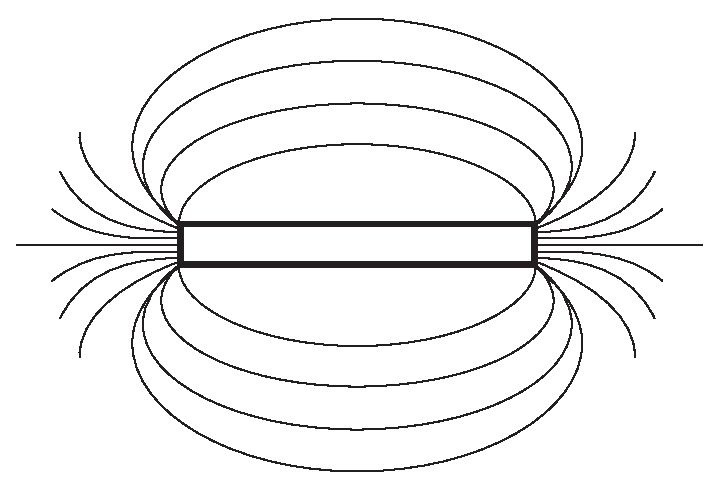
\includegraphics[width=5cm]{../magnet.eps}}
\rput(0,0){\psCoil[coilwidth=1cm,coilheight=0.5]{-1800}{1800}}
\psline(-1.75,0.5)(-2.5,0.5)(-2.5,-4)
\Ucc[labeloffset=0](-2.5,-4)(2.5,-4){A}
\psline(2.5,-4)(2.5,0.5)(1.75,0.5)
\uput[u](0,0.6){\parbox[c]{3cm}{coil with $N$ turns and
cross-sectional area, $A$}} \psline{<-}(4.8,0.4)(5.2,0.4)
\uput[d](5,-2){\parbox[c]{3cm}{magnetic field, $B$ moving to the
left.}}
\rput(3.8,0){\tiny{N}} \rput(6.1,0){\tiny{S}}
\psellipticarcn{->}(-2.8,0)(0.2,0.4){180}{-90}
\uput[l](-3,0){\parbox{1.5cm}{induced current direction}}
\end{pspicture}
\end{center}

When the north pole of a magnet is pushed into a solenoid, the
flux in the solenoid increases so the induced current will have an
associated magnetic field pointing out of the solenoid (opposite
to the magnet's field).  When the north pole is pulled out, the
flux decreases, so the induced current will have an associated
magnetic field pointing into the solenoid (same direction as the
magnet's field) to try to oppose the change. The directions of
currents and associated magnetic fields can all be found using
only the Right Hand Rule. When the fingers of the right hand are
pointed in the direction of the magnetic field, the thumb points in the
direction of the current. When the thumb is pointed in the
direction of the magnetic field, the fingers point in the
direction of the current.

\Tip{An easy way to create a magnetic field of changing
intensity is to move a permanent magnet next to a wire or coil of
wire.  The magnetic field must increase or decrease in intensity
\textit{perpendicular} to the wire (so that the magnetic field lines "cut
across" the conductor), or else no voltage will be induced.}

\Tip{Finding the direction of the induced current}{The induced
current generates a magnetic field. The induced magnetic field is
in a direction that tends to cancel out the change in the magnetic field in the loop of wire. So, you can use the Right Hand Rule to find
the direction of the induced current by remembering that the
induced magnetic field is opposite in direction to the change in the magnetic
field.}

Electromagnetic induction is put into practical use in the
construction of electrical generators, which use mechanical power
to move a magnetic field past coils of wire to generate voltage.
However, this is by no means the only practical use for this
principle.

If we recall that the magnetic field produced by a
current-carrying wire is always perpendicular to the wire, and
that the flux intensity of this magnetic field varies with the
amount of current which passes through it, we can see that a wire is capable of
inducing a voltage \textit{along its own length} if the current is changing. This effect is called
\textit{self-induction}. Self-induction is when a changing magnetic field is produced by
changes in current through a wire, inducing a voltage along the
length of that same wire.

If the magnetic flux is enhanced
by bending the wire into the shape of a coil, and/or wrapping that
coil around a material of high permeability, this effect of
self-induced voltage will be more intense. A device constructed to
take advantage of this effect is called an \textit{inductor}, and
will be discussed in greater detail in the next chapter.

\Extension{Lenz's Law}{The induced current will create a magnetic
field that opposes the change in the magnetic flux.}

\begin{wex}
{Faraday's Law} {Consider a flat square coil with 5 turns. The
coil is 0,50~m on each side, and has a magnetic field of 0,5~T
passing through it. The plane of the coil is perpendicular to the
magnetic field: the field points out of the page. Use Faraday's
Law to calculate the induced emf, if the magnetic field is
increases uniformly from 0,5~T to 1~T in 10~s. Determine the
direction of the induced current.

} {\westep{Identify what is required} We are required to use
Faraday's Law to calculate the induced emf.

\westep{Write Faraday's Law} \nequ{\epsilon=-N\frac{\Delta
\phi}{\Delta t}}

\westep{Solve Problem}
\begin{eqnarray*}
\epsilon&=&-N\frac{\Delta \phi}{\Delta t}\\
&=&-N\frac{\phi_f-\phi_i}{\Delta t}\\
&=&-N\frac{B_f\cdot A-B_i\cdot A}{\Delta t}\\
&=&-N\frac{A(B_f -B_i)}{\Delta t}\\
&=&-(5)\frac{(0,5)^2(1-0,5)}{10}\\
&=&-0,0625~\rm{V}
\end{eqnarray*}
The induced current is anti-clockwise as viewed from the direction of the increasing magnetic field.
}
\end{wex}

\subsection{Real-life applications}
The following devices use Faraday's Law in their operation.
\begin{itemize}
\item{induction stoves}
\item{tape players}
\item{metal detectors}
\item{transformers}
\end{itemize}

\Activity{Research Project}{Real-life applications of Faraday's Law}{
Choose one of the following devices and do some research on the internet or in a library how your device works. You will need to refer to Faraday's Law in your explanation.
\begin{itemize}
\item{induction stoves}
\item{tape players}
\item{metal detectors}
\item{transformers}
\end{itemize}}

\Exercise{Faraday's Law}{
\begin{enumerate}
\item State Faraday's Law in words and write down a mathematical relationship.
\item Describe what happens when a bar magnet is pushed into or pulled out of a solenoid connected to an ammeter. Draw pictures to support your description.
\item Use the Right Hand Rule to determine the direction of the induced current in the solenoid below.
\begin{center}
\begin{pspicture}(-4.8,-4.6)(7.4,2)
%\psgrid
\rput(5,0){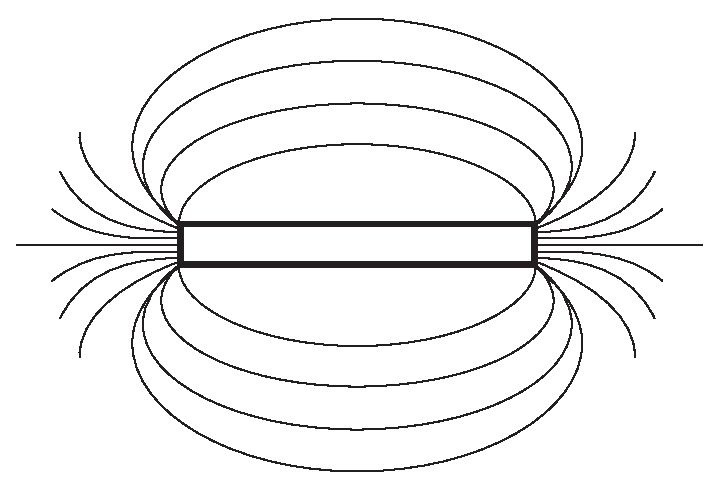
\includegraphics[width=5cm]{../magnet.eps}}
\rput(0,0){\psCoil[coilwidth=1cm,coilheight=0.5]{-1800}{1800}}
\psline(-1.75,0.5)(-2.5,0.5)(-2.5,-4)
\Ucc[labeloffset=0](-2.5,-4)(2.5,-4){A}
\psline(2.5,-4)(2.5,0.5)(1.75,0.5)
\uput[u](0,0.6){\parbox[c]{3cm}{coil with $N$ turns and
cross-sectional area, $A$}} \psline{<-}(4.8,0.4)(5.2,0.4)
\rput(3.8,0){\tiny{S}} \rput(6.1,0){\tiny{N}}
\end{pspicture}
\end{center}
\end{enumerate}
\practiceinfo

\begin{tabular}[h]{cccccc}
(1.) 00u9 & (2.) 00ua & (3.) 00ub & 
 \end{tabular}
}


\section{Transformers}
%\begin{syllabus}
%\item Draw a sketch of the main features of a transformer
%\item Use Faraday's Law to explain how a transformer works in words and pictures.
%\item Use the equation for Faraday's Law to derive an expression involving the ratio between the voltages and number of windings in the primary and secondary coils.
%\item Use the expression Vs/Vp = Ns/Np to perform calculations for transformers with various specifications.
%\item State the difference between a step up and a step down transformer in both structure and function.
%\item Give an example of the use of transformers
%\item Note: The essential features of a transformer are two coils of wire, called the primary and the secondary, which are wound around different sections of the same iron core. When an alternating voltage is applied to the primary coil it creates an alternating current in that coil, which induces an alternating magnetic field in the iron core.  This changing magnetic field induces an emf, which creates a current in the secondary coil.Transformers are very important in the supply of electricity nationally. In order to reduce energy losses due to heating, electrical energy is transported from power stations along power lines at high voltage and low current.  Transformers are used to step the voltage up from the power station to the power lines, and step it down from the power lines to buildings where it is needed.
%\item Additional Suggestions: Give circuit symbol for a transformer
%\item Additional Suggestions: Give a description of transformers in the real-world, link to the power-grid, appliances, etc that use transformers.
%\item Additional Suggestions: Lots of info for interesting facts etc. on wikipedia
%\item Additional Suggestions: At least 2 worked examples using transfromer equations
%\item Additional Suggestions: activity could be: \url{http://en.wikibooks.org/wiki/School_science/How_to_make_a_transformer}
%\end{syllabus}

One of the real-world applications of Faraday's Law is in a
\textit{transformer}.

Eskom generates electricity at around 22~000~V. When you plug in a
toaster, the mains voltage is 220~V. A transformer is used to
\textit{step-down} the high voltage to the lower voltage that is
used as mains voltage.

\Definition{Transformer}{A transformer is an electrical device
that uses the principle of induction between the primary coil and
the secondary coil to either step-up or step-down the voltage.}

The essential features of a transformer are two coils of wire,
called the primary coil and the secondary coil, which are wound around
different sections of the same iron core.

\begin{center}
\begin{pspicture}(-5,-2)(5,2)
%\psgrid[gridcolor=gray]
\psframe[fillcolor=lightgray,fillstyle=solid](-2,-2)(2,2)
\psframe[fillcolor=white,fillstyle=solid](-1,-1)(1,1)
\psframe[linestyle=dashed,linearc=0.5cm](-1.5,-1.5)(1.5,1.5)
\psline(-4,1)(-2,1)
\multirput(0,0)(0,0.2){9}{\psline(-2,-1)(-1,-0.6)}
\psline(-4,-1)(-2,-1)

\psline(4,1)(2,1) \multirput(0,0)(0,0.2){9}{\psline(1,-0.6)(2,-1)}
\psline(4,-1)(2,-1)

\rput(0,1.9){iron core} \uput[u](-3.2,0){primary coil}
\uput[u](3.2,0){secondary coil} \uput{0.1cm}[u](0,-1.5){magnetic
flux}
%\uput[u](0,2){Main features of a transformer}
\end{pspicture}
\end{center}

When an alternating voltage is applied to the primary coil it
creates an alternating current in that coil, which induces an
alternating magnetic field in the iron core.  The changing
magnetic flux through the secondary coil induces an emf, which creates a current in this secondary coil.

The circuit symbol for a transformer is:

\begin{center}
\begin{pspicture}(2.5,2.5)
%\psgrid
\psset{unit=0.5} \pnode(0,5){A} \pnode(0,0){B} \pnode(5,5){C}
\pnode(5,0){D} \transformer(A)(B)(C)(D){$\mathcal T$}
\end{pspicture}
\end{center}

By choosing the number of coils in the secondary solenoid relative to the number of coils in the primary solenoid, we can choose how much bigger or smaller the induced secondary current is by comparison to the current in the primary solenoid (so by how much the current is stepped up or down.)

This ability to transform
voltage and current levels according to a simple ratio, determined
by the ratio of input and output coil turns is a very useful property of transformers and accounts for the name. We can derive a
mathematical relationship by using Faraday's law.

Assume that an alternating voltage ${V_p}$ is applied to the
primary coil (which has $N_p$ turns) of a transformer. The current
that results from this voltage generates a changing magnetic flux $\phi_p$.
We can then describe the emf in the primary coil by: \nequ{V_p =
N_p\frac{\Delta \phi_p}{\Delta t}} Similarly, for the secondary
coil, \nequ{V_s = N_s\frac{\Delta \phi_s}{\Delta t}}

If we assume that the primary and secondary windings are perfectly
coupled, then: \nequ{\phi_p = \phi_s} which means that:
\begin {equation*}
\frac{V_p}{V_s}=\frac{N_p}{N_s}
\end {equation*}

\begin{wex}{Transformer specifications}{Calculate the voltage on the secondary coil if the voltage on the primary coil is 120~V and the ratio of primary windings to secondary windings is 10:1.}{

\westep{Determine how to approach the problem} Use
\begin {equation*}
\frac{V_p}{V_s}=\frac{N_p}{N_s}
\end {equation*}
with
\begin{itemize}
\item $V_p=120$
\item $\frac{N_p}{N_s}=\frac{10}{1}$
\end{itemize}

\westep{Rearrange equation to solve for $V_s$}
\begin{eqnarray*}
\frac{V_p}{V_s}&=&\frac{N_p}{N_s}\\
\frac{1}{V_s}&=&\frac{N_p}{N_s}\frac{1}{V_p}\\
\therefore V_s&=&\frac{1}{\frac{N_p}{N_s}}V_p
\end{eqnarray*}

\westep{Substitute values and solve for $V_s$}
\begin{eqnarray*}
V_s&=&\frac{1}{\frac{N_p}{N_s}}V_p\\
&=&\frac{1}{\frac{10}{1}}120\\
&=&12\;\rm{V}
\end{eqnarray*}

}
\end{wex}


A transformer designed to output more voltage than it takes in
across the input coil is called a \textit{step-up} transformer. A
step-up transformer has more windings on the secondary coil than
on the primary coil. This means that: \nequ{N_s>N_p}

Similarly, a transformer designed to output less than it takes in
across the input coil is called a \textit{step-down} transformer.
A step-down transformer has more windings on the primary coil than
on the primary coil. This means that: \nequ{N_p>N_s}

We use a step-up transformer to increase the voltage from the primary coil to the secondary coil. It is used at power stations to increase the voltage for the transmission lines.
A step-down transformer decreases the voltage from the primary coil to the secondary coil. It is particularly used to decrease the voltage from the transmission lines to a voltage which can be used in factories and in homes.

Transformer technology has made long-range electric power
distribution practical. Without the ability to efficiently step
voltage up and down, it would be cost-prohibitive to construct
power systems for anything but close-range (within a few kilometres) use.

As useful as transformers are, they only work with AC,
not DC. This is because the phenomenon of mutual inductance relies on
\textit{changing} magnetic fields, and direct current (DC) can
only produce steady magnetic fields, transformers simply will not
work with direct current.

Of course, direct current may be
interrupted (pulsed) through the primary winding of a transformer
to create a changing magnetic field (as is done in automotive
ignition systems to produce high-voltage spark plug power from a
low-voltage DC battery), but pulsed DC is not that different from
AC. Perhaps more than any other reason, this is why AC finds such
widespread application in power systems.
% Phet simluation on Faraday's Law: SIYAVULA-SIMULATION:http://cnx.org/content/m38923/latest/#id63458
\simulation{phet on faradays law}{VPlxa}
\subsection{Real-world applications}
Transformers are very important in the supply of electricity
nationally. In order to reduce energy losses due to heating,
electrical energy is transported from power stations along power
lines at high voltage and low current.  Transformers are used to
step the voltage up from the power station to the power lines, and
step it down from the power lines to buildings where it is needed.



\Exercise{Transformers}
\begin{enumerate}
\item Draw a sketch of the main features of a transformer
\item Use Faraday's Law to explain how a transformer works in words and pictures.
\item Use the equation for Faraday's Law to derive an expression involving the ratios of the voltages and the number of windings in the primary and secondary coils.
\item If we have $N_p$ = 100 and $N_s$ = 50, and we connect the primary winding to a 230~V, 50Hz supply, then calculate the voltage on the secondary winding.
\item State the difference between a step-up and a step-down transformer in both structure and function.
\item Give an example of the use of transformers.
\end{enumerate}
% Automatically inserted shortcodes - number to insert 6
\par \practiceinfo
\par \begin{tabular}[h]{cccccc}
% Question 1
(1.)	01hf	&
% Question 2
(2.)	01hg	&
% Question 3
(3.)	01hh	&
% Question 4
(4.)	01hi	&
% Question 5
(5.)	01hj	&
% Question 6
(6.)	01hk	 % End row of shortcodes
\end{tabular}
% Automatically inserted shortcodes - number inserted 6

\section{Motion of a charged particle in a magnetic field}
%\begin{syllabus}
%\item State that when a charged particle moves through a magnetic field it experiences a force.
%\item Use the equation F=qvB to calculate the force exerted on a charge that moves at right angles to a magnetic field.
%\item Use the Right Hand Rule to determine the direction of the force.
%\item Explain how this effect is used in a television
%\item Note: To use the Right Hand Rule to find the direction of the force the magnetic field exerts on the moving charge, point your fingers in the direction of the velocity of the charge and turn them (as if turning a screwdriver) towards the direction of the magnetic field.  Your thumb will point in the direction of the force.  If the charge is negative, the direction of the force will be opposite to the direction of your thumb.By only using the Right Hand Rule in the NCS learners are less likely to get confused than when there are different rules to remember.
%\end{syllabus}

When a charged particle moves through a magnetic field it
experiences a force. For a particle that is moving at right angles
to the magnetic field, the force is given by:
\begin {equation*}
F = qvB
\end {equation*}
where $q$ is the charge on the particle, $v$
is the velocity of the particle and $B$ is the magnetic field
through which the particle is moving. This force is called the Lorentz force.

\begin{center}
\begin{pspicture}(0,0)(8,4)
%\psgrid
%field
\multirput(0.5,0.5)(1.5,0){5}{$\odot$}
\multirput(0.5,1.5)(1.5,0){5}{$\odot$}
\multirput(0.5,2.5)(1.5,0){5}{$\odot$}
\multirput(0.5,3.5)(1.5,0){5}{$\odot$}

\rput(2.3,2.25){$q$}
\psdot[dotscale=2](2,2.25)
\psline{->}(2,2.25)(2,1.5)
\rput(2.2,1.9){$v$}
\psline[linecolor=gray,linestyle=dashed]{->}(2,2.25)(0,2.25)
\rput(1,2){$F$}

\rput(5.8,2.25){$q$}
\psdot[dotscale=2](6,2.25)
\psline{->}(6,2.25)(6,3.5)
\rput(6.2,3){$v$}
\psline[linecolor=gray,linestyle=dashed]{->}(6,2.25)(8,2.25)
\rput(7,2){$F$}


\end{pspicture}
\end{center}

\begin{wex}{Charged particle moving in a magnetic field}{An electron travels at $150 {\rm m.s^{-1}}$ at right angles to a magnetic field of 80~000~T. What force is exerted on the electron? }{
\westep {Determine what is required}
We are required to determine the force on a moving charge in a magnetic field
\westep {Determine how to approach the problem}
We can use the formula:
\begin{equation*}
F = qvB
\end{equation*}
\westep {Determine what is given}
We are given
\begin{itemize}
\item $q = 1,6 \times 10^{-19} {\rm C}$ (The charge on an electron)
\item $v = 150 {\rm m.s^{-1}}$
\item $B = 80~000 {\rm T}$
\end{itemize}
\westep{Determine the force}
\begin{eqnarray*}
F &=& qvB\\
&=& (1,6 \times 10^{-19} {\rm C})(150 {\rm m.s^{-1}})( 80~000 {\rm T})\\
&=& 1,92 \times 10^{-12} {\rm N}
\end{eqnarray*}}
\end{wex}

\Tip{The direction of the force exerted on a charged particle moving
through a magnetic field is determined by using the Right Hand
Rule.\\
Point your first finger (index finger) in the direction of the velocity of the charge, your second finger (middle finger) in the direction of the magnetic field and then your thumb will point in the direction of
the force exerted on the charge.  If the charge is negative, the direction of the force
will be opposite to the direction of your thumb.}

\subsection{Real-world applications}
The following devices use the movement of charge in a magnetic field
\begin{itemize}
\item old televisions (cathode ray tubes)
\item oscilloscope
\end{itemize}

\Activity{Research Project}{Real-life applications of charges moving in a magnetic field}{
Choose one of the following devices and do some research on the internet or in a library how your device works.
\begin{itemize}
\item{oscilloscope}
\item{television}
\end{itemize}}

\Exercise{Lorentz Force}{
\begin{enumerate}
\item What happens to a charged particle when it moves through a magnetic field?
\item Explain how you would use the Right Hand Rule to determine the direction of the force experienced by a charged particle as it moves in a magnetic field.
\end{enumerate}
\practiceinfo

\begin{tabular}[h]{cccccc}
(1.) 00uc & (2.) 00ud & 
 \end{tabular}
}
% Presentation on electromagnetism: SIYAVULA-PRESENTATION:http://cnx.org/content/m38919/latest/#slidesharefigure

\summary{VPmbf}
\begin {enumerate}
\item Electromagnetism is the study of the properties and relationship between electric currents and magnetism.
\item A current-carrying conductor will produce a magnetic field around the conductor.
\item The direction of the magnetic field is found by using the Right Hand Rule.
\item Electromagnets are temporary magnets formed by current-carrying conductors.
\item Electromagnetic induction occurs when a changing magnetic field induces a voltage in a current-carrying conductor.
\item Transformers use electromagnetic induction to alter the voltage.
\item A moving charged particle will experience a force in a magnetic field.
\end {enumerate}

\begin{eocexercises}{}
\begin {enumerate}
\item State the Right Hand Rule to determine the direction of a magnetic field around a current carrying wire and the Right Hand Rule to determine the direction of the force experienced by a moving charged particle in a magnetic field.
\item What did Hans Oersted discover about the relationship between electricity and magnetism?
\item List two uses of electromagnetism.
\item Draw a labelled diagram of an electromagnet and show the poles of the electromagnet on your sketch.
\item Transformers are useful electrical devices.
\begin{enumerate}
\item What is a transformer?
\item Draw a sketch of a step-down transformer.
\item What is the difference between a step-down and step-up transformer?
\item When would you use a step-up transformer?

\end{enumerate}

\item Calculate the voltage on the secondary coil of a transformer if the voltage on the primary coil is 22~000~V and the ratio of primary windings to secondary windings is 500:1.

\item You find a transformer with 1000 windings on the primary coil and 200 windings on the secondary coil.
\begin{enumerate}
\item What type of transformer is it?
\item What will be the voltage on the secondary coil if the voltage on the primary coil is 400~V?

\end{enumerate}
%\item[IEB 2005/11 HG] An electric cable consists of two long straight parallel wires separated by plastic insulating material. Each wire carries a current $I$ in the same direction (as shown in the diagram below).

%\begin{center}
%\begin{pspicture}(0,0)(6,1)
%\SpecialCoor
%\psgrid[gridcolor=lightgray]
%\def\rod{\psellipse[fillcolor=white,fillstyle=solid](0,0.2)(0.1,0.2)
%\psframe[fillcolor=white,fillstyle=solid,linestyle=none](0,0)(2,0.4)
%\psline(0,0)(2,0) \psline(0,0.4)(2,0.4)
%\rput(2,0){\psellipse[fillcolor=white,fillstyle=solid](0,0.2)(0.1,0.2)}}
%\psline[linewidth=1.5pt](0,0.2)(2,0.2) \rput(2,0){\rod}
%\rput(3,0.2){I}\psline{->}(3.2,0.2)(3.8,0.2)
%\psline[linewidth=1.5pt](4,0.2)(6,0.2) \uput[u](1,0.1){Wire B}
%\psline[linewidth=1.5pt](0,0.6)(2,0.6) \rput(2,0.4){\rod}
%\rput(3,0.6){I}\psline{->}(3.2,0.6)(3.8,0.6)
%\psline[linewidth=1.5pt](4,0.6)(6,0.6) \uput[u](1,0.5){Wire A}
%\end{pspicture}
%\end{center}
%Which of the following is \textbf{true} concerning the force of
%Wire A on Wire B?
%\begin{center}
%\begin{tabular}{|c|l|l|}\hline\hline
%&\textbf{Direction of Force}&\textbf{Origin of
%Force}\\\hline\hline (a)&towards A (attraction)&electrostatic
%force between opposite charges\\\hline (b)&towards B
%(repulsion)&electrostatic force between opposite charges\\\hline
%(c)&towards A (attraction)&magnetic force on current-carrying
%conductor\\\hline (d)&towards B (repulsion)&magnetic force on
%current-carrying conductor\\\hline
%\end{tabular}
%\end{center}

%\item[IEB 2005/11 HG1]\textbf{Force of parallel current-carrying conductors}\\
%Two long straight parallel current-carrying conductors placed 1 m
%apart from each other in a vacuum each carry a current of 1 A in
%the same direction.
%\begin{enumerate}
%\item{What is the magnitude of the force of 1 m of one conductor on the other?}
%\item{How does the force compare with that in the previous question when the %current in one of the conductors is halved, and their distance of separation is %halved?}
%\end{enumerate}

\item[IEB 2005/11 HG] An electron moving horizontally in a TV tube enters a region where there is a uniform magnetic field. This causes the electron to move along the path (shown by the solid line) because the magnetic field exerts a constant force on it. What is the direction of this magnetic field?
\begin{center}
\begin{pspicture}(-5,0)(2,6)
\SpecialCoor
%\psgrid[gridcolor=lightgray]
\psplot[plotstyle=curve,arrows=->]{-5}{2}{2 x exp 1.5 add}
\psline(2,0)(2,6) \psline[linestyle=dashed](-5,1.5)(2,1.5)
\uput[l](2,6){TV screen}
\end{pspicture}
\end{center}

\begin{enumerate}
\item{upwards (towards the top of the page)}
\item{downwards (towards the bottom of the page)}
\item{into the page}
\item{out of the page}
\end{enumerate}

\end{enumerate}
\practiceinfo

\begin{tabular}[h]{cccccc}
(1.) 00ue & (2.) 00uf & (3.) 00ug & (4.) 00uh & (5.) 00ui & (6.) 00uj & (7.) 00uk & (8.) 00um & (9.) 00un & (10.) 00up & (11.) 00uq & (12.) 00ur & 
 \end{tabular}
\end{eocexercises}

% CHILD SECTION END



% CHILD SECTION START

